\chapter{State of the Art} % Main chapter title

\label{Chapter3} % Change X to a consecutive number; for referencing this chapter elsewhere, use \ref{ChapterX}

This chapter seeks to provide a summary of existing solutions for remote computer access.
It will not cover specific applications, but rather the protocols that are used to communicate with a remote computer.
Generally speaking, there are two types of solutions that have been developed, software solutions, which are covered in Chapter \ref{sec:SoftwareSolutions} and hardware solutions, which are covered in Chapter \ref{sec:HardwareSolutions}.
Various protocols and implementations are covered in the subsections of those two categories.

\section{Software Solutions}\label{sec:SoftwareSolutions}

While there are many applications in existence that allow a user to remotely control a computer from another location, few of them offer the capabilities required to stream high-performing applications to a remote device.
The following subsections will introduce existing solutions to this problem as well as drawbacks that come with each implementation.


\subsection{Remote Desktop Protocol}\label{subsec:RemoteDesktopProtocol}

Microsoft's Remote Desktop Protocol (RDP), is a protocol that defines communication between a terminal server and terminal server client for multimedia purposes \cite{rdpDocs}.
Coming pre-installed on every Windows machine since Windows XP and with clients available for Windows, Mac, and Linux, RDP is an easy to use solution for remotely accessing Windows machines graphically.

Although it is the built-in solution for Windows machines, it isn't without it's drawbacks.
Firstly, only one graphical session is active at one time while using windows.
This means if a user is logged into the host computer and someone initiates a connection with RDP, the user using the host computer will be logged out.
While this isn't always an issue, sensitive programs that don't take well to being logged out may run into issues.
Secondly, RDP does not support relative mouse movement \cite{burgin_2013}.
This means every mouse input is sent to the host computer as an absolute position on the screen, rather than as a relative distance from it's previous location.
This means any program that moves the user's mouse for them, such as 3D applications with a virtual camera, will be sent the absolute position of the client's mouse.
This will cause the application to detect a large movement of the mouse instantly, which can result in erratic camera movement as the program interprets the mouse moving a large distance every time the cursor is reset to the center of the screen.
Again, while this isn't always an issue, tasks such as 3D modeling and animation or game development cannot be controlled properly.


\subsection{Virtual Network Computing}\label{subsec:VirtualNetworkComputing}

Virtual Network Computing (VNC), is a platform-independent system originally developed by Olivetti \& Oracle Research Labs and later bought and shelved by AT\&T \cite{vncFlavors}.
While the original implementation is no longer used in a wide capacity, the protocol it was developed on has been expanded and improved to become one of the most flexible yet simple ways to control a computer remotely.
VNC can run on any modern operating system, and even a web browser can serve as a VNC client.
It was originally built as the simplest form of remote computer control over LAN, allowing system administrators to control almost any kind of computer with a simple, robust, and extremely compatible system.
However, since its use has gradually outgrown it's original scope, VNC isn't usually the right tool for any job greater than remote system management.
Because of it's simplicity and focus on being as straightforward as possible, VNC is often found to be lacking in terms of security and speed \cite{vncFlavors}.
It is not recommended to use VNC over the internet without some secondary form of security, such as SSL or a secure VPN.


\subsection{Chrome Remote Desktop}\label{subsec:ChromeRemoteDesktop}

Google Chromoting\todoquestion{Should this chapter be called Chromoting? "Chrome Remote Desktop" is the much more recognizable name though}, implemented publicly as Chrome Remote Desktop, is an open source protocol that enables remote desktop control through any web browser running on the Chromium engine \cite{chromotingBuildInstructions}.
It prioritizes low bandwidth usage and ease of access, allowing easy server install on every major desktop operating system, and enables any web browser or mobile device to act as a client.
By employing the VP8 compression format (Most commonly seen in internet video streaming), Chromoting is able to keep network traffic low by only sending a few full images of the server's screen as keyframes and transmitting motion with compressed partial frames \cite{miniorange_chromoting}.
These partial frames are calculated by the server using the difference between the previous and current frame, allowing the server to only send the difference between the two frames.

This save in bandwidth and processing done by the client makes it the perfect solution for Google's ChromeOS laptops coming out around the same time.
These low powered machines were built to be laptops running on the power of a web browser with a link back to more powerful computers when the tasks were too great \cite{upson_sengupta_2012}.
While the protocol works well for remote access, it is limited in certain applications by it's conservative approach to bandwidth usage and reliance on the web browser.


\subsection{Secure Shell Protocol}\label{subsec:SecureShellProtocol}

The Secure Shell Protocol (SSH), is a protocol for securely transmitting data over an insecure network \cite{rfc4251}.
Usually used for remote server management, SSH has become the de facto standard for connecting to a remote computer when nothing more than terminal access is needed.
Paired with the associated SSH file transfer (SFTP) or secure copy (SCP) protocols, SSH provides an incredible amount of flexibility for working with remote computers.
It's largest and most obvious drawback is limited graphical support.
While not a problem for it's traditional use-case, it does limit what high-intensity applications can be used with it.

One recent innovation in remote computing has been the introduction of Remote Development using SSH through the Visual Studio Code IDE.
By opening multiple SSH connections to the host machine at once, Visual Studio Code is able to run the IDE's User interface on the client's machine, and simply send all the written code and commands through to the host machine, utilizing it's power to compile code, run applications, and debug software \cite{vscode_ssh}.
This enables a development experience comparable to working on a local machine by only transmitting the data that is needed over the internet and constructing the visual user interface on the client.
Because of this, high-intensity computational programs such as Artificial Intelligence training and simulation can be run on a powerful host machine and only need to transmit the output to the lower-powered client, but graphical applications are still limited.

\section{Hardware Solutions}\label{sec:HardwareSolutions}

While Hardware solutions are not as popular or widespread as software solutions, there has been some innovation in the field that is worth considering.
Hardware solutions usually focus on building a device that has just enough power to connect and stream data to a remote computer in order to leverage its power for the user to use.


\subsection{Thin Clients}\label{subsec:ThinClients}

As discussed in Section \ref{sec:ThinClients}, Thin Clients are a family of devices commonly seen in the corporate world to allow employees to access data centers and computing clusters from their desks.
Due to their low cost and ease of deployment, they are often the device of choice to enable employees to access the full power of the business' computing infrastructure without needed to purchase a powerful device for each employee.
However, since a typical thin client is a headless device, meaning it doesn't come with a monitor, keyboard, mouse, or other peripherals, they are often less portable as one might think.
A thin client is usually set up once, and then left in that place for as long as a desktop would stay.
Especially with laptop sales on the rise, thin clients do not have the benefit of being more portable than the alternatives.

\subsection{Nvidia Shield and GameStream}\label{subsec:NvidiaShieldAndGameStream}

\begin{wrapfigure}{r}{0.375\textwidth}
  \centering
  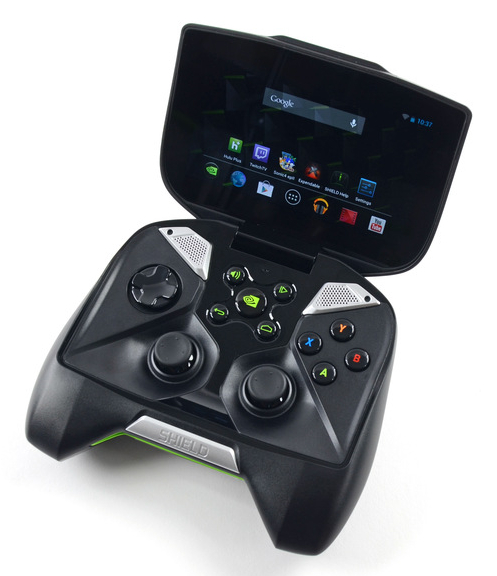
\includegraphics[width=0.3\textwidth]{Figures/nvidia-shield-open-ifixit}
  \caption[Nvidia Shield]{An open Nvidia Shield displaying the home page \cite{ImageNvidiaShield}.}
  \label{fig:nvidiashield}
\end{wrapfigure}

The Nvidia Shield game console was Nvidia's first foray into the realm of remote streaming.
Though it was focused on gaming and media streaming, it was one of the first attempts at using a portable device to stream intensive applications such as games from a host computer \cite{brown_2013}.
At the steep price point of \$349, it definitely was enthusiast hardware for a device that focused on mobile and desktop gaming over running console games or demanding titles locally.
But while the the physical device was praised for performance, battery life, and the experience of streaming games to the console, it didn't perform too well in terms of sales.
It was still widely regarded as a technological breakthrough though, and Nvidia continued to develop the technology into a new device called the Nvidia Shield TV \cite{daniel_2017}.
Focused on bringing the power of a gaming desktop to a TV, the Nvidia Shield TV dropped the idea of portability in favor of filling a different market focused on comfort.
While this is no longer a valid device for the purposes of this paper, the developments of the proprietary GameStream technology that powered the Shield and the Shield TV proved to be even more exciting than the physical devices themselves.

Though the GameStream technology that powers the Nvidia Shield devices is closed source and only officially compatible with the products Nvidia releases, its enticing power and potential drew a community to reverse engineer the protocol.
In 2013, a group of students at Case Western Reserve University developed Moonlight, an open source implementation of the GameStream protocol \cite{moonlight}.
This open source implementation allows the development of GameStream compatible clients that can run on other devices, from other computers to embedded ARM devices.
This stands as a good starting place to develop the solution described in this paper.

\section{Research Questions}\label{sec:ResearchQuestions}

While there are many existing solutions for accessing a computer remotely, many struggle to be performant enough or efficient enough to stream demanding applications to the client without compromising on the user's experience.
This thesis will seek to build a solution that enables the use the power of a desktop computer from a mobile device in a way that is performant and responsive in response to the following questions:

\begin{enumerate}
  \item \textbf{Hardware Feasibility:} \emph{What hardware is needed in order to power a mobile device capable of acting as a client?}
  \item \textbf{Hardware Cost:} \emph{Is it feasible to construct such as device at a lower or comparable cost to existing solutions?}
  \item \textbf{Communication Protocol:} \emph{Does a protocol exist that is efficient enough to stream demanding applications to a client?}
  \item \textbf{Software Application:} \emph{Can a software solution be built to utilize this protocol in a manner that performant enough?}
\end{enumerate}